% Options for packages loaded elsewhere
\PassOptionsToPackage{unicode}{hyperref}
\PassOptionsToPackage{hyphens}{url}
\PassOptionsToPackage{dvipsnames,svgnames,x11names}{xcolor}
%
\documentclass[
  letterpaper,
  DIV=11,
  numbers=noendperiod]{scrartcl}

\usepackage{amsmath,amssymb}
\usepackage{lmodern}
\usepackage{iftex}
\ifPDFTeX
  \usepackage[T1]{fontenc}
  \usepackage[utf8]{inputenc}
  \usepackage{textcomp} % provide euro and other symbols
\else % if luatex or xetex
  \usepackage{unicode-math}
  \defaultfontfeatures{Scale=MatchLowercase}
  \defaultfontfeatures[\rmfamily]{Ligatures=TeX,Scale=1}
\fi
% Use upquote if available, for straight quotes in verbatim environments
\IfFileExists{upquote.sty}{\usepackage{upquote}}{}
\IfFileExists{microtype.sty}{% use microtype if available
  \usepackage[]{microtype}
  \UseMicrotypeSet[protrusion]{basicmath} % disable protrusion for tt fonts
}{}
\makeatletter
\@ifundefined{KOMAClassName}{% if non-KOMA class
  \IfFileExists{parskip.sty}{%
    \usepackage{parskip}
  }{% else
    \setlength{\parindent}{0pt}
    \setlength{\parskip}{6pt plus 2pt minus 1pt}}
}{% if KOMA class
  \KOMAoptions{parskip=half}}
\makeatother
\usepackage{xcolor}
\setlength{\emergencystretch}{3em} % prevent overfull lines
\setcounter{secnumdepth}{5}
% Make \paragraph and \subparagraph free-standing
\ifx\paragraph\undefined\else
  \let\oldparagraph\paragraph
  \renewcommand{\paragraph}[1]{\oldparagraph{#1}\mbox{}}
\fi
\ifx\subparagraph\undefined\else
  \let\oldsubparagraph\subparagraph
  \renewcommand{\subparagraph}[1]{\oldsubparagraph{#1}\mbox{}}
\fi

\usepackage{color}
\usepackage{fancyvrb}
\newcommand{\VerbBar}{|}
\newcommand{\VERB}{\Verb[commandchars=\\\{\}]}
\DefineVerbatimEnvironment{Highlighting}{Verbatim}{commandchars=\\\{\}}
% Add ',fontsize=\small' for more characters per line
\usepackage{framed}
\definecolor{shadecolor}{RGB}{241,243,245}
\newenvironment{Shaded}{\begin{snugshade}}{\end{snugshade}}
\newcommand{\AlertTok}[1]{\textcolor[rgb]{0.68,0.00,0.00}{#1}}
\newcommand{\AnnotationTok}[1]{\textcolor[rgb]{0.37,0.37,0.37}{#1}}
\newcommand{\AttributeTok}[1]{\textcolor[rgb]{0.40,0.45,0.13}{#1}}
\newcommand{\BaseNTok}[1]{\textcolor[rgb]{0.68,0.00,0.00}{#1}}
\newcommand{\BuiltInTok}[1]{\textcolor[rgb]{0.00,0.23,0.31}{#1}}
\newcommand{\CharTok}[1]{\textcolor[rgb]{0.13,0.47,0.30}{#1}}
\newcommand{\CommentTok}[1]{\textcolor[rgb]{0.37,0.37,0.37}{#1}}
\newcommand{\CommentVarTok}[1]{\textcolor[rgb]{0.37,0.37,0.37}{\textit{#1}}}
\newcommand{\ConstantTok}[1]{\textcolor[rgb]{0.56,0.35,0.01}{#1}}
\newcommand{\ControlFlowTok}[1]{\textcolor[rgb]{0.00,0.23,0.31}{#1}}
\newcommand{\DataTypeTok}[1]{\textcolor[rgb]{0.68,0.00,0.00}{#1}}
\newcommand{\DecValTok}[1]{\textcolor[rgb]{0.68,0.00,0.00}{#1}}
\newcommand{\DocumentationTok}[1]{\textcolor[rgb]{0.37,0.37,0.37}{\textit{#1}}}
\newcommand{\ErrorTok}[1]{\textcolor[rgb]{0.68,0.00,0.00}{#1}}
\newcommand{\ExtensionTok}[1]{\textcolor[rgb]{0.00,0.23,0.31}{#1}}
\newcommand{\FloatTok}[1]{\textcolor[rgb]{0.68,0.00,0.00}{#1}}
\newcommand{\FunctionTok}[1]{\textcolor[rgb]{0.28,0.35,0.67}{#1}}
\newcommand{\ImportTok}[1]{\textcolor[rgb]{0.00,0.46,0.62}{#1}}
\newcommand{\InformationTok}[1]{\textcolor[rgb]{0.37,0.37,0.37}{#1}}
\newcommand{\KeywordTok}[1]{\textcolor[rgb]{0.00,0.23,0.31}{#1}}
\newcommand{\NormalTok}[1]{\textcolor[rgb]{0.00,0.23,0.31}{#1}}
\newcommand{\OperatorTok}[1]{\textcolor[rgb]{0.37,0.37,0.37}{#1}}
\newcommand{\OtherTok}[1]{\textcolor[rgb]{0.00,0.23,0.31}{#1}}
\newcommand{\PreprocessorTok}[1]{\textcolor[rgb]{0.68,0.00,0.00}{#1}}
\newcommand{\RegionMarkerTok}[1]{\textcolor[rgb]{0.00,0.23,0.31}{#1}}
\newcommand{\SpecialCharTok}[1]{\textcolor[rgb]{0.37,0.37,0.37}{#1}}
\newcommand{\SpecialStringTok}[1]{\textcolor[rgb]{0.13,0.47,0.30}{#1}}
\newcommand{\StringTok}[1]{\textcolor[rgb]{0.13,0.47,0.30}{#1}}
\newcommand{\VariableTok}[1]{\textcolor[rgb]{0.07,0.07,0.07}{#1}}
\newcommand{\VerbatimStringTok}[1]{\textcolor[rgb]{0.13,0.47,0.30}{#1}}
\newcommand{\WarningTok}[1]{\textcolor[rgb]{0.37,0.37,0.37}{\textit{#1}}}

\providecommand{\tightlist}{%
  \setlength{\itemsep}{0pt}\setlength{\parskip}{0pt}}\usepackage{longtable,booktabs,array}
\usepackage{calc} % for calculating minipage widths
% Correct order of tables after \paragraph or \subparagraph
\usepackage{etoolbox}
\makeatletter
\patchcmd\longtable{\par}{\if@noskipsec\mbox{}\fi\par}{}{}
\makeatother
% Allow footnotes in longtable head/foot
\IfFileExists{footnotehyper.sty}{\usepackage{footnotehyper}}{\usepackage{footnote}}
\makesavenoteenv{longtable}
\usepackage{graphicx}
\makeatletter
\def\maxwidth{\ifdim\Gin@nat@width>\linewidth\linewidth\else\Gin@nat@width\fi}
\def\maxheight{\ifdim\Gin@nat@height>\textheight\textheight\else\Gin@nat@height\fi}
\makeatother
% Scale images if necessary, so that they will not overflow the page
% margins by default, and it is still possible to overwrite the defaults
% using explicit options in \includegraphics[width, height, ...]{}
\setkeys{Gin}{width=\maxwidth,height=\maxheight,keepaspectratio}
% Set default figure placement to htbp
\makeatletter
\def\fps@figure{htbp}
\makeatother

\KOMAoption{captions}{tableheading}
\setmainfont{Times New Roman}
\makeatletter
\makeatother
\makeatletter
\makeatother
\makeatletter
\@ifpackageloaded{caption}{}{\usepackage{caption}}
\AtBeginDocument{%
\ifdefined\contentsname
  \renewcommand*\contentsname{Table of contents}
\else
  \newcommand\contentsname{Table of contents}
\fi
\ifdefined\listfigurename
  \renewcommand*\listfigurename{List of Figures}
\else
  \newcommand\listfigurename{List of Figures}
\fi
\ifdefined\listtablename
  \renewcommand*\listtablename{List of Tables}
\else
  \newcommand\listtablename{List of Tables}
\fi
\ifdefined\figurename
  \renewcommand*\figurename{Figure}
\else
  \newcommand\figurename{Figure}
\fi
\ifdefined\tablename
  \renewcommand*\tablename{Table}
\else
  \newcommand\tablename{Table}
\fi
}
\@ifpackageloaded{float}{}{\usepackage{float}}
\floatstyle{ruled}
\@ifundefined{c@chapter}{\newfloat{codelisting}{h}{lop}}{\newfloat{codelisting}{h}{lop}[chapter]}
\floatname{codelisting}{Listing}
\newcommand*\listoflistings{\listof{codelisting}{List of Listings}}
\makeatother
\makeatletter
\@ifpackageloaded{caption}{}{\usepackage{caption}}
\@ifpackageloaded{subcaption}{}{\usepackage{subcaption}}
\makeatother
\makeatletter
\@ifpackageloaded{tcolorbox}{}{\usepackage[many]{tcolorbox}}
\makeatother
\makeatletter
\@ifundefined{shadecolor}{\definecolor{shadecolor}{rgb}{.97, .97, .97}}
\makeatother
\makeatletter
\makeatother
\ifLuaTeX
  \usepackage{selnolig}  % disable illegal ligatures
\fi
\usepackage[]{biblatex}
\addbibresource{references.bib}
\IfFileExists{bookmark.sty}{\usepackage{bookmark}}{\usepackage{hyperref}}
\IfFileExists{xurl.sty}{\usepackage{xurl}}{} % add URL line breaks if available
\urlstyle{same} % disable monospaced font for URLs
\hypersetup{
  pdftitle={Segregate The Variability Climate Is Responsible For In Vegetation Loss},
  pdfauthor={Kalong Boniface; Fugah Seletey Mitchell},
  colorlinks=true,
  linkcolor={blue},
  filecolor={Maroon},
  citecolor={blue},
  urlcolor={Blue},
  pdfcreator={LaTeX via pandoc}}

\title{Segregate The Variability Climate Is Responsible For In
Vegetation Loss}
\usepackage{etoolbox}
\makeatletter
\providecommand{\subtitle}[1]{% add subtitle to \maketitle
  \apptocmd{\@title}{\par {\large #1 \par}}{}{}
}
\makeatother
\subtitle{Quantifying The Status of Galamsey With Time Series Analsis}
\author{Kalong Boniface \and Fugah Seletey Mitchell}
\date{2022-08-24}

\begin{document}
\maketitle
\ifdefined\Shaded\renewenvironment{Shaded}{\begin{tcolorbox}[frame hidden, sharp corners, enhanced, interior hidden, borderline west={3pt}{0pt}{shadecolor}, boxrule=0pt, breakable]}{\end{tcolorbox}}\fi

\renewcommand*\contentsname{Table of Contents}
{
\hypersetup{linkcolor=}
\setcounter{tocdepth}{2}
\tableofcontents
}
\hypertarget{chapter-one}{%
\section{CHAPTER ONE}\label{chapter-one}}

\hypertarget{introduction}{%
\subsection{INTRODUCTION}\label{introduction}}

The purpose of this paper is to establish an understanding in time
series analysis on remotely sensed data. Which will introduced us to the
fundamentals of time series modeling, including decomposition,
autocorrelation and modeling historical changes in Galamsey Operation in
Ghana, the Cause,Dangers and it's Environmental impact.

Galamsey also known as ``gather them and
sell'',\autocite{owusu-nimo2018} is the term given by local Ghanaian for
illegal small-scale gold mining in Ghana . The major cause of Galamsey
is unemployment among the youth in Ghana \autocite{gracia2018}. Young
university graduates rarely find work and when they do it hardly
sustains them. The result is that these youth go the extra mile to earn
a living for themselves and their family.

Another factor is that lack of job security. On November 13, 2009 a
collapse occurred in an illegal, privately owned mine in Dompoase, in
the Ashanti Region of Ghana. At least 18 workers were killed, including
13 women, who worked as porters for the miners. Officials described the
disaster as the worst mine collapse in Ghanaian history
\autocite{womendi2009} .

Illegal mining causes damage to the land and water supply
\autocite{ansah2017} . In March 2017, the Minister of Lands and Natural
Resources, Mr.~John Peter Amewu, gave the Galamsey operators/illegal
miners a three-week ultimatum to stop their activities or be prepared to
face the law \autocite{allotey2017} . The activities by Galamseyers have
depleted Ghana's forest cover and they have caused water pollution, due
to the crude and unregulated nature of the mining process
\autocite{gyekye} .

Under current Ghanaian constitution, it is illegal to operate as
galamseyer.That is to dig on land granted to mining companies as
concessions or licenses and any other land in search for gold. In some
cases, Galamseyers are the first to discover and work extensive gold
deposits before mining companies find out and take over. Galamseyers are
the main indicator of the presence of gold in free metallic dust form or
they process oxide or sulfide gold ore using liquid mercury.

Between 20,000 to 50,000, including thousands from China are believed to
be engaged in Galamsey in Ghana.But according to the Information
Minister 200,000 and nearly 3 million people, recently are now into
Galamsey operation and rely on it for their livelihoods \autocite[
]{goldgu2017}. Their operations are mostly in the southern part of Ghana
where it is believe to have substantial reserves of gold deposits,
usually within the area of large mining companies
\autocite{barenblitt2021} . As a group, they are economically
disadvantaged. Galamsey settlements are usually poorer than neighboring
agricultural villages. They have high rates of accidents and are exposed
to mercury poisoning from their crude processing methods. Many women are
among the workers, acting mostly as porters for the miners.

\hypertarget{background-of-the-study}{%
\subsubsection{Background of The Study}\label{background-of-the-study}}

As Galamsey is considered an illegal activity, they operations are
hidden to the eyes of the authorities.So locating them is quite tricky
,but with satellite imagery ,it now possible to locate their operating
and put an end to it. One of the features of Google Earth Engine is the
ability to access years of satellite imagery without needing to
download, organize, store and process this information. For instance,
within the Satellite image

collection, now it possible to access imagery back to the 90's, allowing
us to look at areas of interest on the map to visualize and quantify how
much things has changed over time. With Earth Engine, Google maintains
the data and offers it's computing power for processing.Users can now
access hundreds of time series images and analyze changes across decades
using GIS and R or other programming language to analyze these datasets.

\hypertarget{problem-statement}{%
\subsubsection{Problem Statement}\label{problem-statement}}

The Footprint of Galamsey is Spreading at a very faster rate, causing
vegetation loss.Other factors accounting to vegetation loss may largely
include climate change,urban and exurban development, bush fires. But
not much works or research has been done to tell the extent to which
Galamsey causes vegetation loss. This research attempts to segregate the
variability climate is responsible for in vegetation loss so as to
attribute the residual variability to Galamsey and other related
activities such as bush-fires etc.

\hypertarget{research-questions}{%
\subsubsection{Research Questions}\label{research-questions}}

To address the challenge of the vegetation variability in this work, the
following several statements were formed:

\begin{itemize}
\item
  Are there any changes in vegetation cause by Galamsey and Climate
  change in Ghana?
\item
  Is there any relationship between vegetation and land surface
  temperature in Ghana?
\end{itemize}

\hypertarget{research-objectives}{%
\subsubsection{Research Objectives}\label{research-objectives}}

The purpose is to establish an understanding in time series analysis on
remotely sensed data. We will be introduced to the fundamentals of time
series modeling, including decomposition, autocorrelation and modeling
historical changes.

\begin{itemize}
\item
  Perform time series analysis on satellite derived vegetation indices
\item
  Estimate the extent to which Galamsey causes vegetation loss in Ghana.
\item
  Dissociate or single out the variability climate is responsible for in
  vegetation loss
\end{itemize}

\hypertarget{significance-of-the-study}{%
\subsubsection{Significance Of The
Study}\label{significance-of-the-study}}

There are significant changes in vegetation cover in Ghana over the past
30 years, and these dynamics are related strongly to climatic factors
such as temperature and other factors. Examining the effects of climatic
change on Ghana's vegetation during thirty years.

This study allows us to explore climatic differences and climate-related
drivers thanks to this study. Additionally, it offers a chance to
research how climatic variability affects the ecosystem and human
health. By merging climate and vegetation variation utilizing NDVI, LST,
and EVI data to understand the relationship between vegetation and
climate change under tropical climate conditions, it closes research
gaps in Ghana.

\hypertarget{scope-of-the-study}{%
\subsubsection{Scope of The Study}\label{scope-of-the-study}}

\hypertarget{limitation-of-the-study}{%
\subsubsection{Limitation Of The Study}\label{limitation-of-the-study}}

The goal of time series modeling is to employ the simplest model
feasible to account for as much data as possible while still developing
an explanatory model of the data that does not overfit the issue set.

Remote sensing data has additional limits that make this more difficult
when dividing time series data into component pieces. It is almost
certain that data from distant sensing will not provide the same level
of precision.

Additionally, atmospheric factors can distort the visual findings,
causing the vegetation's color to shift dramatically from image to image
as a result of atmospheric factors (fog, ground moisture, cloud cover).

\hypertarget{organization-of-the-study}{%
\subsubsection{Organization of The
Study}\label{organization-of-the-study}}

\hypertarget{chapter-two}{%
\section{CHAPTER TWO}\label{chapter-two}}

\hypertarget{literature-review}{%
\subsection{LITERATURE REVIEW}\label{literature-review}}

\hypertarget{theoretical-review}{%
\subsubsection{Theoretical Review}\label{theoretical-review}}

This literature review will follow narrative approach to gain insight
into research topic. A time series is a set of observations, each being
recorded at a particular time and the collection of such observation is
referred to as time series data. The data is analysed to extract
statistical information, characteristics of the data and to predict the
output. As the data might tend to follow a pattern in time series data,
the Machine Learning model finds it difficult to predict appropriately
hence time series analysis and its approaches have made it simpler for
prediction. The methods used and results from those methods achieved by
former researchers will be summarized including different methods on
time series and comparing them with each other.

\hypertarget{what-is-time-series-analysis}{%
\paragraph{What is Time Series
Analysis?}\label{what-is-time-series-analysis}}

Makridakis and hibon, in time series analysis researchers have conducted
a competition named M-competition in 1987 , Where participants could
submit their forecasting on 1001 time series data taken from demography,
industry, and economics. There were four main findings from the
competition were:

\begin{itemize}
\item
  Statistically sophisticated or complex methods do not necessarily
  provide more accurate forecasts than simpler ones.
\item
  The relative ranking of the performance of the various methods varies
  according to the accuracy measure being used.
\item
  The accuracy when various methods are being combined outperformed, on
  average, the individual methods being combined and does very well in
  comparison to other methods.
\item
  The accuracy of the various methods depends upon the length of the
  forecasting horizon involved.
\end{itemize}

The time series data is visualized and analyzed to find out mainly three
things, trend, seasonality, and Heteroscedasticity.

\textbf{Trend:} It can be defined as the observation of increasing or
decreasing pattern over a period. In a stationary time series, mean of
the time series data must be constant in time and whereas in general
time series the mean is arbitrary function of time.

Seasonality: It refers to a cyclic happening of events. A pattern which
repeats itself after a period.

\textbf{Heteroscedasticity:} It is also known as level; it is defined as
the non-constant variance from the mean calculated at different time
periods.

Few methods do not perform well in forecasting if the data is seasonal,
and few do not perform well with trends in the data. Hence trends,
seasonality and heteroscedasticity must be considered to select the best
statistical method in forecasting.

\hypertarget{time-series-forecasting-using-stochastic-models}{%
\paragraph{\texorpdfstring{\textbf{Time Series Forecasting Using
Stochastic
Models}}{Time Series Forecasting Using Stochastic Models}}\label{time-series-forecasting-using-stochastic-models}}

The selection of a proper model is extremely important as it reflects
the underlying structure of the series and this fitted model in turn is
used for future forecasting. A time series model is said to be linear or
non-linear depending on whether the current value of the series is a
linear or non-linear function of past observations.

In general models for time series data can have many forms and represent
different stochastic processes. There are two widely used linear time
series models in literature.

\emph{Autoregressive (AR)} and \emph{Moving Average (MA)} models,
combining these two, the Autoregressive Moving Average (ARMA) and
\emph{Autoregressive Integrated Moving Average (ARIMA)} models have been
proposed in many literature. The \emph{Autoregressive Fractionally
Integrated Moving Average (ARFIMA)} model generalizes ARMA and ARIMA
models. For seasonal time series forecasting, a variation of ARIMA. The
\emph{Seasonal Autoregressive Integrated Moving Average (SARIMA)} {]}
model is used.

ARIMA model and its different variations are based on the famous
Box-Jenkins principle {[}6, 8,12, 23{]} and so these are also broadly
known as the Box-Jenkins models.

Linear models have drawn much attention due to their relative simplicity
in understanding and implementation. However many practical time series
show non-linear patterns. For example, as mentioned by R. Parrelli in
{[}28{]}, non-linear models are appropriate for predicting volatility
changes in economic and financial time series. Considering these facts,
various non-linear models have been suggested in literature. Some of
them are the famous Autoregressive Conditional Heteroskedasticity (ARCH)
{[}9, 28{]} model and its variations like Generalized ARCH (GARCH) {[}9,
28{]}, Exponential Generalized ARCH (EGARCH) {[}9{]} etc., the Threshold
Autoregressive (TAR) {[}8, 10{]} model, the Non-linear Autoregressive
(NAR) {[}7{]} model, the Non-linear Moving Average (NMA) {[}28{]} model,
All the methods consider either of trend, seasonality, or
heteroscedasticity to predict the future output. Time series data must
be decomposed based on the findings from data analysis. Based on the
findings from analysis data must be broken into trend or seasonality.

\hypertarget{exponential-smoothing-models}{%
\subparagraph{Exponential Smoothing
Models:}\label{exponential-smoothing-models}}

Time-series data relies on the assumption that the observation at a
certain point of time depends on previous observations in time . The
previous observations are given weights as they contribute to the future
prediction. The process of weighting is done using a notation called
`Theta' (Cryer, J.D., 1986). To find the best possible value for theta,
we must perform sum of squared errors between the actual versus
predicted value of the previous observation. Using this process, we can
predict the next value but to predict more than one value this process
does contribute much as the prediction as going to be same as the
previous value.

To understand the methods and to evaluate different models, few concepts
like \emph{stationarity} and \emph{differencing} must be understood.
Both these concepts help in making the core concepts of the methods easy
to interpret.

\hypertarget{stationarity}{%
\subparagraph{\texorpdfstring{\textbf{Stationarity:}}{Stationarity:}}\label{stationarity}}

Stationarity alludes to an irregular process that creates a time-series
which has mean, and distribution to be constant through time.
Distribution only depends on time and not location in time (Manuca, R.
and Savit, R., 1996). If the distribution is same over different time
windows is strong stationarity and if only mean and variance are
similar, then it is weak stationarity. Irrespective of strong or weak,
stationarity helps build a class of models such Autoregression (AR),
Moving Average (MA), ARIMA (Witt, A., Kurths, J. and Pikovsky, A.,
1998).

An MA(q) process is always stationary, irrespective of the values the MA
parameters {[}23{]}. The conditions regarding stationarity and
invertibility of AR and MA processes also hold for an ARMA process. An
ARMA(p, q) process is stationary if all the roots of the characteristic
equation \(\phi (L) = 0\) lie outside the unit circle. Similarly, if all
the roots of the lag equation

\(\theta (L) = 0\) lie outside the unit circle, then the ARMA(p, q)
process is invertible and can be expressed as a pure AR process..

\hypertarget{differencing}{%
\subparagraph{\texorpdfstring{\textbf{Differencing:}}{Differencing:}}\label{differencing}}

This concept is used to make trending and seasonal data stationary.
Subtraction between current observation and previous observation is the
process of differencing. It helps in making the mean constant (Dickey,
D.A. and Pantula, S.G., 1987).

\hypertarget{autoregressive-models-ar}{%
\subparagraph{\texorpdfstring{\textbf{Autoregressive models
(AR):}}{Autoregressive models (AR):}}\label{autoregressive-models-ar}}

AR work on a concept called lags which is defined as the forecast of a
series is solely based on the past values in the series (Cryer, J.D.,
1986). Formula for Autoregression AR(1):
\(\displaystyle y_{t} = \omega + \phi Y _{t-1}+ e_{t}\) is stationary
when \$ \textbar{}\phi\_\{1\}\textbar{} \textless{} 1,\$ with a constant
mean \(\displaystyle \mu = \frac{\omega}{1-\phi_{1}}\) and constant
variance
\(\displaystyle \gamma_{o} = \frac{\sigma^{2}}{1-\phi_{1}^{2}}\) Where ;
\quad    \(y_{t}\) = Target ,\quad \(\omega\) = Intercept,\quad \(\phi\)
= Coefficient,\quad \(Y_{t-1}\)=Lagged target,\quad \(e_{t}\) =
Error\textbackslash{}

It depends only on one lag in the past and also called AR model of order
one (Shibata, R., 1976). Autoregressive models are also known as long
memory models as they must keep the memory of all the lags until its
initial start point and must calculate their value. If there is any
shock incident in the past which must have led to fluctuations in the
data, it will have its effect on the present value which makes the model
quite sensitive to shocks (Shibata, R., 1976).

\hypertarget{moving-average-ma}{%
\subparagraph{\texorpdfstring{\textbf{Moving Average
(MA):}}{Moving Average (MA):}}\label{moving-average-ma}}

The moving average model forecasts a series based on the past error in
the series called error lags. Hunter, J.S., Formula for moving average
method is given as:\(y_{t} = \omega + \theta e _{t-1}+ e_{t}\)

In (2), all the abbreviations are same to AR model formula except, =
Previous error

There arises a question as this method uses the error for the previous
value but when it reaches to the first point there will be no previous
value, to overcome this the average of the series is considered as the
value before the starting point. These are short memory models as the
error in the past will not have much effect on the future value (Hunter,
J.S., 1986).

\hypertarget{comparing-ar-method-with-ma-method}{%
\subparagraph{\texorpdfstring{\textbf{Comparing AR method with MA
method:}}{Comparing AR method with MA method:}}\label{comparing-ar-method-with-ma-method}}

Let focus on the two methods which were used in the early years of time
series forecasting and compare the performance of each model on a
particular task. Testing against general autoregressive and moving
average error models where the regressors include lagged dependent
variables. (Godfrey, L.G., 1978) In their paper have explained the order
of the error process under the alternate hypothesis using lagrange
multiplier test (Silvey, S.D., 1959). As per the tests the errors of
both the models were similar, but the constraints were different under
which the tests were performed are also to be considered. As they have
concluded in their paper stating that that the outcome of the model's
performance depends on the estimate chosen to be null hypothesis or
alternate hypothesis.

In addition, paper written by (Baltagi, B.H. and Li, Q., 1995),
Demonstrates the comparison of AR and MA model using Burke, Godfrey, and
Termayne test. To the error component model. They explained choosing of
this test is because these are simple to implement as they only require
within residual or OLS residual (Baltagi, B.H. and Li, Q., 1995). The
outcome of the experiment was explained as when the test used within
residual AR model performed well but had problems, if the test used OLS
residual MA model performance was good. They have concluded stating that
MA will performance much better when the parameters are changed.

The findings of both the paper were quite different but one cannot prove
either of the model to be better as the performance depends on the
parameters used in the model. Each model is unique to its use case, and
it depends on the user to choose accordingly based on the data.

\hypertarget{autocorrelation-and-partial-autocorrelation-functions-acf-and-pacf}{%
\subparagraph{\texorpdfstring{\textbf{Autocorrelation and Partial
Autocorrelation Functions (ACF and
PACF)}}{Autocorrelation and Partial Autocorrelation Functions (ACF and PACF)}}\label{autocorrelation-and-partial-autocorrelation-functions-acf-and-pacf}}

To determine a proper model for a given time series data, it is
necessary to carry out the ACF and PACF analysis. These statistical
measures reflect how the observations in a time series are related to
each other. For modeling and forecasting purpose it is often useful to
plot the ACF and PACF against consecutive time lags. These plots help in
determining the order of AR and MA terms. For a time series
\({x(t),t = 0,1, 2,...}\)the Autocovariance {[}21, 23{]} at lag k is
defined as:

\(\mu\) is the mean of the time series,
i.e.~\(\mu = E\left[x_{t}\right]\). The autocovariance at lag zero
i.e.~\(y_{0}\) is the variance of the time series. From the definition
it is clear that the autocorrelation coefficient \$ p\_\{k\}\$ is
dimensionless and so is independent of the scale of measurement. Also,
clearly \(-1 \leq p\_{k}\leq 1\). Statisticians Box and Jenkins {[}6{]}
termed \(y_{k }\) as the theoretical Autocovariance Function (ACVF) and
\(p_{k}\) as the theoretical Autocorrelation Function (ACF).

Another measure, known as the Partial Autucorrelation Function (PACF) is
used to measure the correlation between an observation k period ago and
the current observation, after controlling for observations at
intermediate lags (i.e.~at lags \textless{} k ) {[}12{]}. At lag 1,
PACF(1) is same as ACF(1). The detailed formulae for calculating PACF
are given in {[}6, 23{]}.

Normally, the stochastic process governing a time series is unknown and
so it is not possible to determine the actual or theoretical ACF and
PACF values. Rather these values are to be estimated from the training
data, i.e.~the known time series at hand. The estimated ACF and PACF
values from the training data are respectively termed as sample ACF and
PACF {[}6, 23{]}.

As given in {[}23{]}, the most appropriate sample estimate for the ACVF
at lag k is ACF plot is useful in determining the type of model to fit
to a time series of length N. Since ACF is symmetrical about lag zero,
it is only required to plot the sample ACF for positive lags, from lag
one on-wards to a maximum lag of about N/4. The sample PACF plot helps
in identifying the maximum order of an AR process.

\hypertarget{autoregressive-moving-average-arma-model}{%
\subparagraph{\texorpdfstring{\textbf{Autoregressive Moving Average
(ARMA)
model:}}{Autoregressive Moving Average (ARMA) model:}}\label{autoregressive-moving-average-arma-model}}

ARMA model is a combination of AR and MA models. The equation of the AR
model of order one, when it reaches to the starting point will have
infinite moving average (Choi, B., 2012). In ARMA model p and q have to
defined, where p = number of significant terms in ACF and q = number of
significant terms in PACF.

To determine the optimal value for p and q there are two ways:

\begin{itemize}
\item
  Plotting patterns in correlation
\item
  Automatic selection techniques
\end{itemize}

\hypertarget{plotting-patterns-in-correlation}{%
\paragraph{\texorpdfstring{\textbf{Plotting patterns in
correlation:}}{Plotting patterns in correlation:}}\label{plotting-patterns-in-correlation}}

There are two functions used for plotting patterns in correlation:

\hypertarget{auto-correlation-factor-acf}{%
\subparagraph{\texorpdfstring{\textbf{Auto correlation factor
(ACF):}}{Auto correlation factor (ACF):}}\label{auto-correlation-factor-acf}}

It is the correlation between the observations at the current time stamp
and observations at the previous time stamp (Hagan, M.T. and Behr, S.M.,
1987).

\hypertarget{partial-auto-correlation-factor-pacf}{%
\subparagraph{\texorpdfstring{\textbf{Partial auto correlation factor
(PACF):}}{Partial auto correlation factor (PACF):}}\label{partial-auto-correlation-factor-pacf}}

The correlation between the observations at two different time stamps,
assuming both observations are correlated to the observations at another
time stamp (Hagan, M.T. and Behr, S.M., 1987).

\hypertarget{automatic-selection-techniques}{%
\paragraph{\texorpdfstring{\textbf{Automatic selection
techniques:}}{Automatic selection techniques:}}\label{automatic-selection-techniques}}

There are three commonly used techniques for automatic selection of time
series model:

\hypertarget{minimum-info-criteria-minic}{%
\subparagraph{\texorpdfstring{\textbf{Minimum info criteria
(MINIC):}}{Minimum info criteria (MINIC):}}\label{minimum-info-criteria-minic}}

This builds multiple combinations of models across a grid search of AR
and MA terms. It then finds the model with lowest Bayesian information
criteria (Stadnytska, T., Braun, S. and Werner, J., 2008).

\begin{itemize}
\item
  \textbf{Squared canonical correlations (SCAN):} It looks at
  correlation matrix of the data, then it compares it with its lags. It
  then looks at the eigen values from the correlation matrix to find the
  combination of AR and MA probably having SCAN as 0. It finds the pair
  as the best where the convergence is quickest (Stadnytska, T., Braun,
  S. and Werner, J., 2008).
\item
  \textbf{The extended sample auto correlation function (ESACF):} As it
  is known that AR and MA are related. Essentially it filters out the AR
  terms until only MA piece is left. This process is repeated until
  fewest AR terms are left and maximum MA terms (Stadnytska, T., Braun,
  S. and Werner, J., 2008).
\end{itemize}

It completely depends on the individual to choose from either of the
methods helping them to find the optimal value of p and q for better
performance of the model.

\hypertarget{autoregressive-integrated-moving-average-arima}{%
\paragraph{\texorpdfstring{\textbf{Autoregressive Integrated Moving
average
(ARIMA):}}{Autoregressive Integrated Moving average (ARIMA):}}\label{autoregressive-integrated-moving-average-arima}}

To understand ARIMA model, we need to understand ARMA model as this is
just an extension to ARMA model. Essentially, we need to make data
stationary to feed it to a machine learning model. It is done by through
differencing. ARIMA models are mathematically written as ARIMA(p,d,q),
where p and q are same as ARMA model but d = number of first differences
(Yu, G. and Zhang, C., 2004, May).

\hypertarget{seasonal-autoregressive-integrated-moving-average-sarima}{%
\paragraph{\texorpdfstring{\textbf{Seasonal Autoregressive Integrated
Moving Average
(SARIMA):}}{Seasonal Autoregressive Integrated Moving Average (SARIMA):}}\label{seasonal-autoregressive-integrated-moving-average-sarima}}

SARIMA models were introduced to handle seasonality in the data.
Seasonality is different from stationarity; however, seasonality can be
handled using stationarity up to some extent, but seasonal correlations
cannot be eliminated completely. SARIMA models are mathematically
written as SARIMA\((p,d,q)(P,D,Q)^{s}\).

Where;

P = Number of seasonal AR terms, D = Number of seasonal differences, Q =
Number of seasonal MA terms, s = Length of the season.

Removing seasonality will help the model to perform better but getting
rid of seasonality in data is a difficult task to do.

\hypertarget{comparing-arima-method-with-sarima-method}{%
\paragraph{\texorpdfstring{\textbf{Comparing ARIMA method with SARIMA
method:}}{Comparing ARIMA method with SARIMA method:}}\label{comparing-arima-method-with-sarima-method}}

In comparison to ARIMA and SARIMA, (Valipour, M., 2015) investigated it
on long-term runoff forecasting in the United States. The results have
shown that SARIMA models have performed better than ARIMA model.
However, it was seen that SARIMA models were very sensitive and a slight
change in a parameter would result in poor performance of the model.

(Wang, S., Li, C. and Lim, A., 2019) have used ARIMA and SARIMA models
from the perspective of Linear System Analysis, Spectra Analysis and
Digital Filtering. It was shown that ARIMA and SARIMA both have not
performed well and the researchers were forced to look beyond these
models for better performance. They have mentioned that ARMA-SIN model
was better but have also said it is relatively difficult to study and
understand the concepts compared to ARIMA and SARIMA model.

The findings from the (Valipour, M., 2015) have proven SARIMA to better
however, their claim contradicts when it was to be compared with the
findings of (Wang, S., Li, C. and Lim, A., 2019). The use of a
particular method must be based on the data, after the analysis it is
known if that the data has trend, they must choose ARIMA and if the data
has seasonality, choosing SARIMA would be helpful.

\hypertarget{advantages-and-disadvantages-of-time-series-forecasting}{%
\paragraph{\texorpdfstring{\textsc{\textbf{ADVANTAGES AND DISADVANTAGES
OF TIME SERIES
FORECASTING}}}{ADVANTAGES AND DISADVANTAGES OF TIME SERIES FORECASTING}}\label{advantages-and-disadvantages-of-time-series-forecasting}}

\textbf{Advantages of time series forecasting:}

\begin{itemize}
\item
  Time series forecasting is of high accuracy and simplicity.
\item
  It can be used to analyze how the changes associated with the data
  point picked correlate with changes in other variables during the same
  time span.
\item
  Statistical techniques have been developed to analyze time series in
  such a way that the factor that influences the fluctuation of the
  series may be identified and handled.
\item
  It can give good output with less variables. As regression models fail
  with less variables, time series models will work better and
  effectively.
\end{itemize}

\textbf{Disadvantages of time series forecasting:}

\begin{itemize}
\item
  Time series models can easily be overfitted, which lead to false
  results.
\item
  It works well with short term forecasting but does not work well with
  long term forecasting.
\item
  It is sensible to outliers, if the outliers are not handled properly
  then it could lead to wrong predictions.
\item
  The different elements that impact the fluctuations of a series cannot
  be fully adjusted by the time series analysis
\end{itemize}

\hypertarget{time-series-forecasting-using-support-vector-machines}{%
\paragraph{\texorpdfstring{\textbf{Time Series Forecasting Using Support
Vector
Machines}}{Time Series Forecasting Using Support Vector Machines}}\label{time-series-forecasting-using-support-vector-machines}}

\hypertarget{concept-of-support-vector-machines}{%
\subparagraph{\texorpdfstring{\textbf{Concept of Support Vector
Machines}}{Concept of Support Vector Machines}}\label{concept-of-support-vector-machines}}

Till now, we have studied about various stochastic and neural network
methods for time series modeling and forecasting. Despite of their own
strengths and weaknesses, these methods are quite successful in
forecasting applications. Recently, a new statistical learning theory,
viz.~the Support Vector Machine (SVM) has been receiving increasing
attention for classification and forecasting {[}18, 24, 30, 31{]}. SVM
was developed by Vapnik and his co-workers at the AT \& T Bell
laboratories in 1995 {[}24, 29, 33{]}. Initially SVMs were designed to
solve pattern classification problems, such as optimal character
recognition, face identification and text classification, etc. But soon
they found wide applications in other domains, such as function
approximation, regression estimation and time series prediction problems
{[}24, 31, 34{]}.

Vapnik's SVM technique is based on the Structural Risk Minimization
(SRM) principle {[}24, 29, 30{]}. The objective of SVM is to find a
decision rule with good generalization ability through selecting some
particular subset of training data, called support vectors {[}29, 31,
33{]}. In this method, an optimal separating hyperplane is constructed,
after non-linearly mapping the input space into a higher dimensional
feature space. Thus, the quality and complexity of SVM solution does not
depend directly on the input space {[}18, 19{]}.

Another important characteristic of SVM is that here the training
process is equivalent to solving a linearly constrained quadratic
programming problem. So, contrary to other networks' training, the SVM
solution is always unique and globally optimal. However a major
disadvantage of SVM is that when the training size is large, it requires
an enormous amount of computation which increases the time complexity of
the solution {[}24{]}.

\hypertarget{forecast-performance-measures}{%
\paragraph{Forecast Performance
Measures}\label{forecast-performance-measures}}

While applying a particular model to some real or simulated time series,
first the raw data is divided into two parts, viz.~the Training Set and
Test Set. The observations in the training set are used for constructing
the desired model. Often a small subpart of the training set is kept for
validation purpose and is known as the Validation Set. Sometimes a
preprocessing is done by normalizing the data or taking logarithmic or
other transforms. One such famous technique is the Box-Cox
Transformation {[}23{]}. Once a model is constructed, it is used for
generating forecasts. The test set observations are kept for verifying
how accurate the fitted model performed in forecasting these values. If
necessary, an inverse transformation is applied on the forecasted values
to convert them in original scale. In order to judge the forecasting
accuracy of a particular model or for evaluating and comparing different
models, their relative performance on the test dataset is considered.

Due to the fundamental importance of time series forecasting in many
practical situations, proper care should be taken while selecting a
particular model. For this reason, various performance measures are
proposed in literature {[}3, 7, 8, 9, 24, 27{]} to estimate forecast
accuracy and to compare different models. These are also known as
performance metrics {[}24{]}. Each of these measures is a function of
the actual and forecasted values of the time series.

\hypertarget{description-of-various-forecast-performance-measures}{%
\subparagraph{Description of Various Forecast Performance
Measures}\label{description-of-various-forecast-performance-measures}}

In each of the forthcoming definitions, \(y_{t }\) is the actual value,
\(f_{t}\) is the forecasted value, \(e_{t} = y_{t} - f_{t}\) is the
forecast error and n is the size of the test set. Also,
\(\displaystyle \bar{y} = \frac{1}{n}\sum_{t=1}^{n}y_{t}\) is the test
mean and
\(\displaystyle \sigma^{2} = \frac{1}{n-1}\sum_{t=1}^{n}(y_{t}-\bar{y})^{2}\)is
the test variance.

The Mean Forecast Error (MFE)

This measure is defined as {[}24{]}
\(\displaystyle MFE = \frac{1}{n}\sum_{t=1}^{n}e_{t}\) The properties of
MFE are:

\hypertarget{empirical-review}{%
\subsubsection{Empirical Review}\label{empirical-review}}

LULC data are records that documents to what extent a region is covered
by wetlands, forests, agriculture, impervious surfaces, and other land
and water forms. These water forms include open water or wetlands. Land
use shows how people use landscape either for conservation, development,
agriculture or mixed uses {[}6, 7{]}. Changes In land can be identified
by analysing satellite imagery. However, land use cannot be identified
from satellite imagery. Satellite imagery give us information that helps
in understanding the present landscape. Furthermore, to see changes
through time, different years are needed. With this information, we can
assess decades of data as well as insight into the possible effects of
these changes that has occured and make better decisions before they can
cause great harm. According to {[}10{]}, five different types of LULC
pattern were classified barren lands such as Galamsey Site, agricultural
lands, urban lands, quarries, and free water bodies, to detect the
25years LULC change in the western Nile delta of Egypt. Supervised
maximum likelihood classification (MLC) method together with landsat
images were used in Erdas Imagine software. The finding shows a
significant change in barren land changing into agricultural land
continuously from 1984 to 2009.

Similarly, in {[}1{]} used the maximum likelihood algorithm (MLA) and
Markov chain model (MCA) to study the LULC classification using ArcGIS
and future prediction using Idiri respectively in Kathmandu city Nepal.
Built-up, water body, forest area, open field and cultivated land
classes classified. Results show built-up area significantly increased,
and water body, forest area, open field and cultivated land decrease
downward trend from 1976 to 2009. Furthermore, the Markov chain Analysis
prediction for 2017 shows that in 2017 Urban area will increase to cover
72.24 \(\%\) of the total land in Kathmandu and cultivated land remains
only 20.90\(\%\). Waterbody and the open field will increase
respectively by 0.59\(\%\), 0.19\(\%\) whereas forest land decrease by
0.47\(\%\).

Furthermore, in {[}10{]}, They made used of the Maximum likelihood
classification (MLC), Change detection and spatial matrix analysis to
analyse land cover change of fifty-year period (1954 to 2004) in
Avellino Italy. The result shows 4 LULC classes, with urban land use
increasing rapidly affecting the cultivated land mostly, while woodland
and grassland cover decrease was at a lower rate. Moreover, in {[}11{]}
studied the LULC changes and structure in Dhaka metropolitan, Bangladesh
in a period of 1975 to 2005. Maximum Likelihood Classification (MLC) and
transition matrix method were used for LULC classification and pattern
of LULC. The Result shows six classes in LULC of the water body,

vegetation, bare soil, cultivated land built-up and wetland/lowland.
Also, a significant increase in the built-up land, while cultivated
land, vegetation and wetland decreased accordingly from 1975 to 2005.

Also, {[}12{]} used Maximum Likelihood Classification and comparison
method to study the LULC classification and change respectively from
1976 to 2003 in Tirupati, India. The results show 6 LULC classes,
agricultural land, built-up, dense forest, plantation, water spread and
other land, a significant increase in built-up area, plantation forests
and other land, while a decrease on the part of the waterbody, dense
forest and agricultural land was noticed.

Moreover, in {[}13{]} studied the LULC change in Duzce plain Turkey.
Supervised classification and the Corine land cover nomenclature methods
used. The result shows 5 LULC classes as urban fabric, forest,
heterogeneous agricultural land, inland wasteland and (Industrial,
commercial, and transport) units with an accuracy assessment between
92.41\(\%\) and 97.3\(\%\) for LULC map 2010 and 1987 respectively.
Also, a significant change in LULC was noticed with 11.2\(\%\) increase
in agricultural area and 335\(\%\) decrease of forest land.

Also, a significant increase and a decrease of LULC were noticed between
the years 1973, 1985, and 2000 within the classes.

\begin{Shaded}
\begin{Highlighting}[]
\FunctionTok{library}\NormalTok{(openintro)  }\CommentTok{\# for data}
\end{Highlighting}
\end{Shaded}

\begin{verbatim}
Warning: package 'openintro' was built under R version 4.1.3
\end{verbatim}

\begin{verbatim}
Warning: package 'airports' was built under R version 4.1.3
\end{verbatim}

\begin{verbatim}
Warning: package 'cherryblossom' was built under R version 4.1.3
\end{verbatim}

\begin{verbatim}
Warning: package 'usdata' was built under R version 4.1.3
\end{verbatim}

\begin{Shaded}
\begin{Highlighting}[]
\CommentTok{\#library(tidyverse)  \# for data wrangling and visualization}
\FunctionTok{library}\NormalTok{(knitr)      }\CommentTok{\# for tables}
\end{Highlighting}
\end{Shaded}

\begin{verbatim}
Warning: package 'knitr' was built under R version 4.1.3
\end{verbatim}

\begin{Shaded}
\begin{Highlighting}[]
\FunctionTok{library}\NormalTok{(broom)      }\CommentTok{\# for model summary}
\end{Highlighting}
\end{Shaded}

\begin{verbatim}
Warning: package 'broom' was built under R version 4.1.3
\end{verbatim}

\begin{Shaded}
\begin{Highlighting}[]
\ControlFlowTok{if}\NormalTok{(}\SpecialCharTok{!}\FunctionTok{require}\NormalTok{(}\StringTok{"pacman"}\NormalTok{))\{}\FunctionTok{install.packages}\NormalTok{(}\StringTok{"pacman"}\NormalTok{)\}}
\end{Highlighting}
\end{Shaded}

\begin{verbatim}
Warning: package 'pacman' was built under R version 4.1.3
\end{verbatim}

\begin{Shaded}
\begin{Highlighting}[]
\NormalTok{pacman}\SpecialCharTok{::}\FunctionTok{p\_load}\NormalTok{(}\AttributeTok{char =} \FunctionTok{c}\NormalTok{(}\StringTok{\textquotesingle{}rgee\textquotesingle{}}\NormalTok{,}\StringTok{\textquotesingle{}reticulate\textquotesingle{}}\NormalTok{,}\StringTok{\textquotesingle{}raster\textquotesingle{}}\NormalTok{,}\StringTok{\textquotesingle{}tidyverse\textquotesingle{}}\NormalTok{,}
                \StringTok{\textquotesingle{}dplyr\textquotesingle{}}\NormalTok{,}\StringTok{\textquotesingle{}sf\textquotesingle{}}\NormalTok{,}\StringTok{\textquotesingle{}mapview\textquotesingle{}}\NormalTok{,}\StringTok{\textquotesingle{}mapeddit\textquotesingle{}}\NormalTok{,}\StringTok{\textquotesingle{}caret\textquotesingle{}}\NormalTok{,}\StringTok{\textquotesingle{}forcats\textquotesingle{}}\NormalTok{,}\StringTok{\textquotesingle{}reticulate\textquotesingle{}}\NormalTok{,}
                \StringTok{\textquotesingle{}rgee\textquotesingle{}}\NormalTok{, }\StringTok{\textquotesingle{}remotes\textquotesingle{}}\NormalTok{, }\StringTok{\textquotesingle{}magrittr\textquotesingle{}}\NormalTok{, }\StringTok{\textquotesingle{}tigris\textquotesingle{}}\NormalTok{, }\StringTok{\textquotesingle{}tibble\textquotesingle{}}\NormalTok{, }\StringTok{\textquotesingle{}stars\textquotesingle{}}\NormalTok{,                       }\StringTok{\textquotesingle{}stars\textquotesingle{}}\NormalTok{,}
                \StringTok{\textquotesingle{}st\textquotesingle{}}\NormalTok{, }\StringTok{\textquotesingle{}lubridate\textquotesingle{}}\NormalTok{, }\StringTok{\textquotesingle{}imputeTS\textquotesingle{}}\NormalTok{, }\StringTok{\textquotesingle{}leaflet\textquotesingle{}}\NormalTok{, }\StringTok{\textquotesingle{}classInt\textquotesingle{}}\NormalTok{,                            }\StringTok{\textquotesingle{}RColorBrewer\textquotesingle{}}\NormalTok{,}
                \StringTok{\textquotesingle{}ggplot2\textquotesingle{}}\NormalTok{, }\StringTok{\textquotesingle{}googledrive\textquotesingle{}}\NormalTok{, }\StringTok{\textquotesingle{}geojsonio\textquotesingle{}}\NormalTok{, }\StringTok{\textquotesingle{}ggpubr\textquotesingle{}}\NormalTok{,}\StringTok{\textquotesingle{}cartogram\textquotesingle{}}\NormalTok{),}
               \AttributeTok{install =}\NormalTok{ F, }\AttributeTok{update =}\NormalTok{ F, }\AttributeTok{character.only =}\NormalTok{ T)}
\end{Highlighting}
\end{Shaded}

\begin{verbatim}
Warning in pacman::p_load(char = c("rgee", "reticulate", "raster", "tidyverse", : Failed to install/load:
tidyverse, mapeddit
\end{verbatim}

\begin{Shaded}
\begin{Highlighting}[]
\FunctionTok{library}\NormalTok{(rgee)}

\FunctionTok{library}\NormalTok{(reticulate)}
\CommentTok{\#ee\_install()}
\FunctionTok{ee\_check}\NormalTok{()}

\FunctionTok{ee\_Initialize}\NormalTok{(}\StringTok{"kalong"}\NormalTok{,}\AttributeTok{drive =} \ConstantTok{TRUE}\NormalTok{) }\CommentTok{\# initialize GEE,}
\end{Highlighting}
\end{Shaded}

\begin{verbatim}
Auto-refreshing stale OAuth token.
\end{verbatim}

\begin{Shaded}
\begin{Highlighting}[]
\CommentTok{\#this will have you log in to Google Drive}
\end{Highlighting}
\end{Shaded}

\begin{Shaded}
\begin{Highlighting}[]
\FunctionTok{library}\NormalTok{(}\StringTok{\textquotesingle{}sf\textquotesingle{}}\NormalTok{)}
\CommentTok{\# Load shape file}

\CommentTok{\#setwd("C:/Users/Guy/Documents/GitHub/Artisanal{-}Mining{-}In{-}Ghana{-}Galamsey/New Regions")}
\NormalTok{aoi }\OtherTok{\textless{}{-}} \FunctionTok{read\_sf}\NormalTok{(}\StringTok{\textquotesingle{}Ghana shp file/GHA/gadm41\_GHA\_1.shp\textquotesingle{}}\NormalTok{)}
\NormalTok{aoi }\OtherTok{\textless{}{-}} \FunctionTok{st\_transform}\NormalTok{(aoi, }\FunctionTok{st\_crs}\NormalTok{(}\DecValTok{4326}\NormalTok{))}
\NormalTok{aoi.ee }\OtherTok{\textless{}{-}} \FunctionTok{st\_bbox}\NormalTok{(aoi) }\SpecialCharTok{\%\textgreater{}\%}
\FunctionTok{st\_as\_sfc}\NormalTok{() }\SpecialCharTok{\%\textgreater{}\%}
\FunctionTok{sf\_as\_ee}\NormalTok{() }\CommentTok{\#Converts it to an Earth Engine Object}
\end{Highlighting}
\end{Shaded}

\begin{Shaded}
\begin{Highlighting}[]
\NormalTok{getQABits }\OtherTok{\textless{}{-}} \ControlFlowTok{function}\NormalTok{(image, qa) \{}
  \CommentTok{\# Convert binary (character) to decimal (little endian)}
\NormalTok{  qa }\OtherTok{\textless{}{-}} \FunctionTok{sum}\NormalTok{(}\DecValTok{2}\SpecialCharTok{\^{}}\NormalTok{(}\FunctionTok{which}\NormalTok{(}\FunctionTok{rev}\NormalTok{(}\FunctionTok{unlist}\NormalTok{(}\FunctionTok{strsplit}\NormalTok{(}\FunctionTok{as.character}\NormalTok{(qa), }\StringTok{""}\NormalTok{)) }\SpecialCharTok{==} \DecValTok{1}\NormalTok{))}\SpecialCharTok{{-}}\DecValTok{1}\NormalTok{))}
  \CommentTok{\# Return a mask band image, giving the qa value.}
\NormalTok{  image}\SpecialCharTok{$}\FunctionTok{bitwiseAnd}\NormalTok{(qa)}\SpecialCharTok{$}\FunctionTok{lt}\NormalTok{(}\DecValTok{1}\NormalTok{)}
\NormalTok{\}}

\NormalTok{mod.clean }\OtherTok{\textless{}{-}} \ControlFlowTok{function}\NormalTok{(img) \{}
  \CommentTok{\# Extract the NDVI band}
\NormalTok{  ndvi\_values }\OtherTok{\textless{}{-}}\NormalTok{ img}\SpecialCharTok{$}\FunctionTok{select}\NormalTok{(}\StringTok{"EVI"}\NormalTok{)}
  \CommentTok{\# Extract the quality band}
\NormalTok{  ndvi\_qa }\OtherTok{\textless{}{-}}\NormalTok{ img}\SpecialCharTok{$}\FunctionTok{select}\NormalTok{(}\StringTok{"SummaryQA"}\NormalTok{)}
  \CommentTok{\# Select pixels to mask}
\NormalTok{  quality\_mask }\OtherTok{\textless{}{-}} \FunctionTok{getQABits}\NormalTok{(ndvi\_qa, }\StringTok{"11"}\NormalTok{)}
  \CommentTok{\# Mask pixels with value zero.}

  \CommentTok{\#0.0001 is the MODIS Scale Factor}
\NormalTok{  ndvi\_values}\SpecialCharTok{$}\FunctionTok{updateMask}\NormalTok{(quality\_mask)}\SpecialCharTok{$}\FunctionTok{divide}\NormalTok{(ee}\SpecialCharTok{$}\NormalTok{Image}\SpecialCharTok{$}\FunctionTok{constant}\NormalTok{(}\DecValTok{10000}\NormalTok{))}
\NormalTok{\}}

\NormalTok{modis.evi }\OtherTok{\textless{}{-}}\NormalTok{ ee}\SpecialCharTok{$}\FunctionTok{ImageCollection}\NormalTok{(}\StringTok{"MODIS/006/MOD13Q1"}
\NormalTok{                                )}\SpecialCharTok{$}\FunctionTok{filter}\NormalTok{(ee}\SpecialCharTok{$}\NormalTok{Filter}\SpecialCharTok{$}\FunctionTok{date}\NormalTok{(}\StringTok{\textquotesingle{}2000{-}01{-}01\textquotesingle{}}\NormalTok{,}\StringTok{\textquotesingle{}2022{-}01{-}01\textquotesingle{}}\NormalTok{))}\SpecialCharTok{$}\FunctionTok{map}\NormalTok{(mod.clean)}
\end{Highlighting}
\end{Shaded}

Now we will create a hexagonal grid over the study area

\begin{Shaded}
\begin{Highlighting}[]
\FunctionTok{library}\NormalTok{(tibble)}
\NormalTok{aoi.proj }\OtherTok{\textless{}{-}} \FunctionTok{st\_transform}\NormalTok{(aoi, }\FunctionTok{st\_crs}\NormalTok{(}\DecValTok{2392}\NormalTok{))}
\NormalTok{hex }\OtherTok{\textless{}{-}} \FunctionTok{st\_make\_grid}\NormalTok{(}\AttributeTok{x =}\NormalTok{ aoi.proj, }\AttributeTok{cellsize =} \DecValTok{17280}\NormalTok{, }\AttributeTok{square =} \ConstantTok{FALSE}\NormalTok{) }\SpecialCharTok{\%\textgreater{}\%}
\FunctionTok{st\_sf}\NormalTok{() }\SpecialCharTok{\%\textgreater{}\%}
\FunctionTok{rowid\_to\_column}\NormalTok{(}\StringTok{\textquotesingle{}hex\_id\textquotesingle{}}\NormalTok{)}
\NormalTok{hex }\OtherTok{\textless{}{-}}\NormalTok{ hex[aoi.proj,]}
\FunctionTok{plot}\NormalTok{(hex)}
\end{Highlighting}
\end{Shaded}

\begin{figure}[H]

{\centering 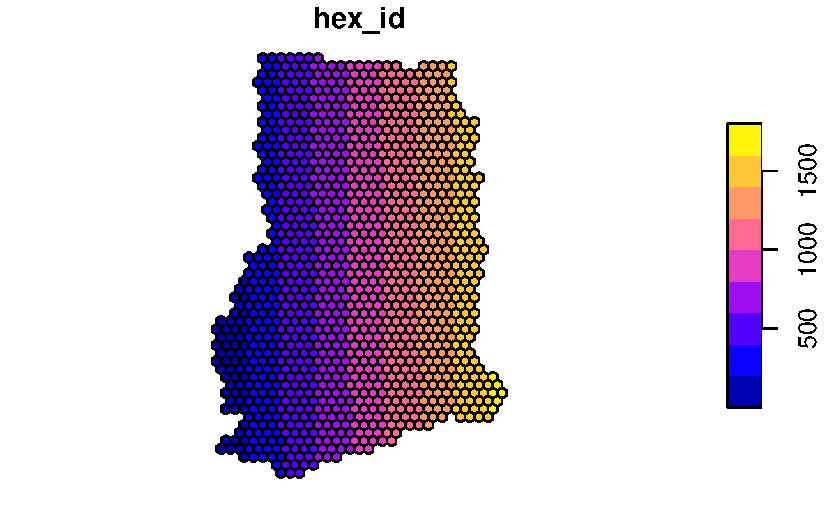
\includegraphics{Quarto_files/figure-pdf/unnamed-chunk-5-1.pdf}

}

\end{figure}

Now we will use the grid created above to extract the mean EVI values
within each cell for the years 2000-2020.

Which we are going to perform a time series analysis on the data within
each grid cell. But first, we will work through the procedure one step
at a time.

\begin{Shaded}
\begin{Highlighting}[]
\CommentTok{\#converting the data to a transposed data frame}
\NormalTok{tsv }\OtherTok{\textless{}{-}} \FunctionTok{data.frame}\NormalTok{(}\AttributeTok{evi =} \FunctionTok{t}\NormalTok{(evi.df[i, }\DecValTok{2}\SpecialCharTok{:}\FunctionTok{ncol}\NormalTok{(evi.df)]))}
\FunctionTok{colnames}\NormalTok{(tsv) }\OtherTok{\textless{}{-}} \FunctionTok{c}\NormalTok{(}\StringTok{"evi"}\NormalTok{)}
\FunctionTok{write.csv}\NormalTok{(tsv,}\StringTok{"Data/tsv.csv"}\NormalTok{)}
\FunctionTok{head}\NormalTok{(tsv) }\CommentTok{\#let\textquotesingle{}s take a look}
\end{Highlighting}
\end{Shaded}

\begin{verbatim}
                 evi
2001-01-17 0.3103816
2001-03-22 0.6017811
2001-04-23 0.5585050
2002-01-17 0.3728227
2002-02-02 0.4369971
2002-04-07 0.5701539
\end{verbatim}

\begin{Shaded}
\begin{Highlighting}[]
\CommentTok{\#}
\CommentTok{\# : My Caption \{tbl{-}letters\}}
\CommentTok{\#}
\CommentTok{\# See @tbl{-}letters.}
\end{Highlighting}
\end{Shaded}

\hypertarget{chapter-three}{%
\section{CHAPTER THREE}\label{chapter-three}}

\hypertarget{methodology}{%
\subsection{METHODOLOGY}\label{methodology}}

Data from a time series is a set of observations made in a particular
order over a period of time. There is a chance for correlation between
observations because time series data points are gathered at close
intervals. To help machine learning classifiers work with time series
data, we provide several new tools. We first contend that local features
or patterns in time series can be found and combined to address
challenges involving time-series categorization. Then, a method to
discover patterns that are helpful for classification is suggested. We
combine these patterns to create computable categorization rules. In
order to mask low-quality pixels, we will first collect Sentinel 2 data
from Google Earth Engine in order to choose NDVI and EVI values.

Instead of analyzing the imagery directly, we will summarize the mean
NDVI and EVI values. This will shorten the analysis time while still
providing an attractive and useful map. We will apply a smoothing
strategy using an ARIMA function to fix the situation where some cells
may not have NDVI and EVI for a particular month. Once NA values have
been eliminated, the time series will be divided to eliminate
seasonality before the normalized data is fitted using a linear model.
We will go to classify our data on the map and map it after we have
extracted the linear trend.

\hypertarget{research-design}{%
\subsection{Research Design}\label{research-design}}

In this study, the submission used a quantitative approach. Instead of
using subjective judgment, findings and conclusions heavily rely on the
use of statistical methods and reliable time series models.

\hypertarget{specification-of-the-model}{%
\subsubsection{Specification of the
Model}\label{specification-of-the-model}}

\hypertarget{data-representation}{%
\subsubsection{Data Representation}\label{data-representation}}

The site in which the experimental plots of this study will be installed
is the Garamba National Park
(\href{https://www.scirp.org/journal/paperinformation.aspx?paperid=112855\#f1}{Figure
1}) with an area of 4900 km\textsuperscript{2} is located in the
Northwest ofAfrica, and shares its northern border with b. The 4900
km\textsuperscript{2} Garamba National Park is located in the north-east
of the Democratic Republic of Congo, and shares its northern border with
South Sudan; 3??45'N - 4??41'N, 28??48'E - 30??00'E, altitude: 710 -
1061 m; framed by the 29\textsuperscript{th} and West meridians, while,
from South to North, it stretches between parallels 3??8' and 4??4'
North, over an area estimated at 4900 km\textsuperscript{2} by the
gravimetric method.

\hypertarget{section}{%
\subsubsection{}\label{section}}

The Analysis Of Variance (ANOVA) Method

\hypertarget{the-empirical-theory-model}{%
\subsubsection{The Empirical * Theory
model}\label{the-empirical-theory-model}}

\hypertarget{assumptions}{%
\subsubsection{Assumptions}\label{assumptions}}

\begin{Shaded}
\begin{Highlighting}[]
\CommentTok{\#We want to get an idea of the number of entries with no EVI value}
\NormalTok{na.cnt }\OtherTok{\textless{}{-}} \FunctionTok{length}\NormalTok{(tsv[}\FunctionTok{is.na}\NormalTok{(tsv)])}
\NormalTok{evi.trend}\SpecialCharTok{$}\NormalTok{na.cnt[i] }\OtherTok{\textless{}{-}}\NormalTok{ na.cnt}
\NormalTok{td }\OtherTok{\textless{}{-}}\NormalTok{ tsv }\SpecialCharTok{\%\textgreater{}\%}
  \FunctionTok{mutate}\NormalTok{(}\AttributeTok{month =} \FunctionTok{month}\NormalTok{(}\FunctionTok{as.Date}\NormalTok{(}\FunctionTok{rownames}\NormalTok{(tsv))), }\AttributeTok{year =} \FunctionTok{year}\NormalTok{(}\FunctionTok{as.Date}\NormalTok{(}\FunctionTok{rownames}\NormalTok{(tsv)))) }\SpecialCharTok{\%\textgreater{}\%}
  \FunctionTok{group\_by}\NormalTok{(year, month) }\SpecialCharTok{\%\textgreater{}\%}
  \FunctionTok{summarise}\NormalTok{(}\AttributeTok{mean\_evi =} \FunctionTok{mean}\NormalTok{(evi, }\AttributeTok{na.rm =}\NormalTok{ T), }\AttributeTok{.groups =} \StringTok{"keep"}\NormalTok{) }\SpecialCharTok{\%\textgreater{}\%}
  \FunctionTok{as.data.frame}\NormalTok{()}
\FunctionTok{head}\NormalTok{(td)}
\end{Highlighting}
\end{Shaded}

\begin{verbatim}
  year month  mean_evi
1 2001     1 0.3103816
2 2001     3 0.6017811
3 2001     4 0.5585050
4 2002     1 0.3728227
5 2002     2 0.4369971
6 2002     4 0.6160278
\end{verbatim}

That looks better! Unfortunately though, there are a number of dates
which don't have any evi value at all, let's figure out which ones these
are.

\begin{Shaded}
\begin{Highlighting}[]
\NormalTok{dx}\SpecialCharTok{$}\NormalTok{mean\_evi }\OtherTok{\textless{}{-}} \ConstantTok{NA}
\NormalTok{tdx }\OtherTok{\textless{}{-}} \FunctionTok{rbind}\NormalTok{(td, dx) }\SpecialCharTok{\%\textgreater{}\%}
  \FunctionTok{arrange}\NormalTok{(date)}
\FunctionTok{write.csv}\NormalTok{(tdx,}\StringTok{"Data/tdx.csv"}\NormalTok{)}
\NormalTok{tdx }\OtherTok{\textless{}{-}} \FunctionTok{read.csv}\NormalTok{(}\StringTok{"Data/tdx.csv"}\NormalTok{)}
\FunctionTok{head}\NormalTok{(tdx)}
\end{Highlighting}
\end{Shaded}

\begin{verbatim}
    X year month  mean_evi       date
1   1 2001     1 0.3103816 2001-01-01
2 216 2001     2        NA 2001-02-01
3   2 2001     3 0.6017811 2001-03-01
4   3 2001     4 0.5585050 2001-04-01
5 510 2001     5        NA 2001-05-01
6 610 2001     6        NA 2001-06-01
\end{verbatim}

\begin{Shaded}
\begin{Highlighting}[]
\NormalTok{na.cnt }\OtherTok{\textless{}{-}} \FunctionTok{length}\NormalTok{(tdx[}\FunctionTok{is.na}\NormalTok{(tdx)])}
\CommentTok{\# Convert data to time series.}
\NormalTok{tdx }\OtherTok{\textless{}{-}} \FunctionTok{ts}\NormalTok{(}\AttributeTok{data =}\NormalTok{ tdx}\SpecialCharTok{$}\NormalTok{mean\_evi, }\AttributeTok{start =} \FunctionTok{c}\NormalTok{(}\DecValTok{2001}\NormalTok{, }\DecValTok{1}\NormalTok{), }\AttributeTok{end =} \FunctionTok{c}\NormalTok{(}\DecValTok{2019}\NormalTok{, }\DecValTok{11}\NormalTok{), }\AttributeTok{frequency =} \DecValTok{12}\NormalTok{)}
\FunctionTok{plot}\NormalTok{(tdx)}
\end{Highlighting}
\end{Shaded}

\begin{figure}[H]

{\centering 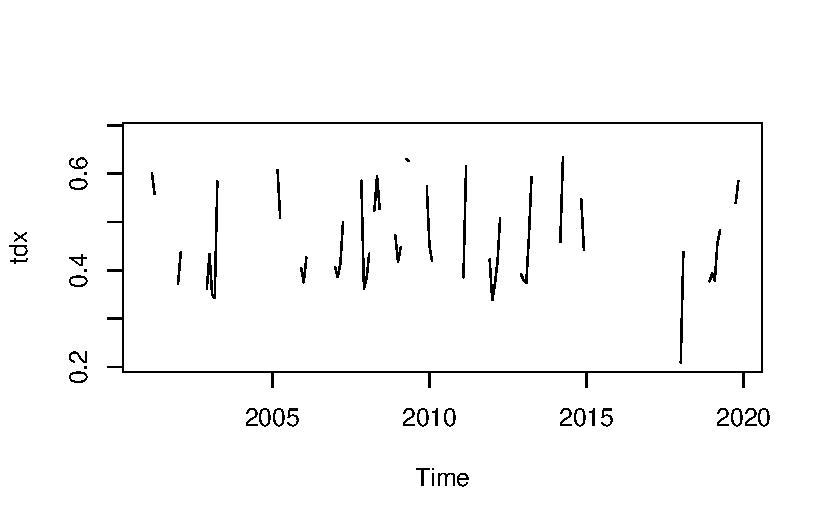
\includegraphics{Quarto_files/figure-pdf/unnamed-chunk-12-1.pdf}

}

\end{figure}

\begin{Shaded}
\begin{Highlighting}[]
\FunctionTok{library}\NormalTok{(imputeTS)}
\NormalTok{tdx }\OtherTok{\textless{}{-}} \ControlFlowTok{if}\NormalTok{(na.cnt }\SpecialCharTok{\textgreater{}} \DecValTok{0}\NormalTok{)\{imputeTS}\SpecialCharTok{::}\FunctionTok{na\_kalman}\NormalTok{(tdx, }\AttributeTok{model =} \StringTok{"auto.arima"}\NormalTok{, }\AttributeTok{smooth =}\NormalTok{ T)\} }\ControlFlowTok{else}\NormalTok{ \{}
\NormalTok{    tdx}
\NormalTok{\}}
\FunctionTok{plot}\NormalTok{(tdx)}
\end{Highlighting}
\end{Shaded}

\begin{figure}[H]

{\centering 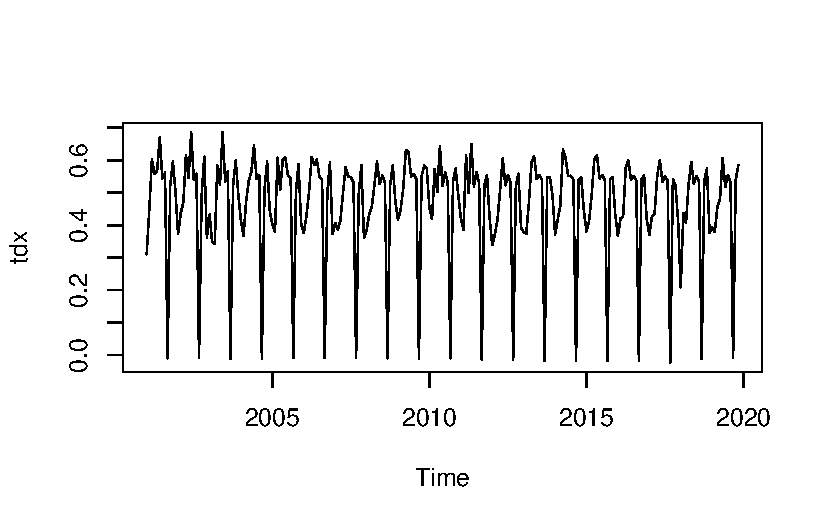
\includegraphics{Quarto_files/figure-pdf/unnamed-chunk-13-1.pdf}

}

\end{figure}

\begin{Shaded}
\begin{Highlighting}[]
\NormalTok{new\_tdx }\OtherTok{\textless{}{-}} \FunctionTok{write.csv}\NormalTok{(tdx,}\StringTok{"Data/new\_tdx.csv"}\NormalTok{)}
\end{Highlighting}
\end{Shaded}

\begin{Shaded}
\begin{Highlighting}[]
\NormalTok{tdx.dcp }\OtherTok{\textless{}{-}} \FunctionTok{stl}\NormalTok{(tdx, }\AttributeTok{s.window =} \StringTok{\textquotesingle{}periodic\textquotesingle{}}\NormalTok{)}
\FunctionTok{plot}\NormalTok{(tdx.dcp)}
\end{Highlighting}
\end{Shaded}

\begin{figure}[H]

{\centering 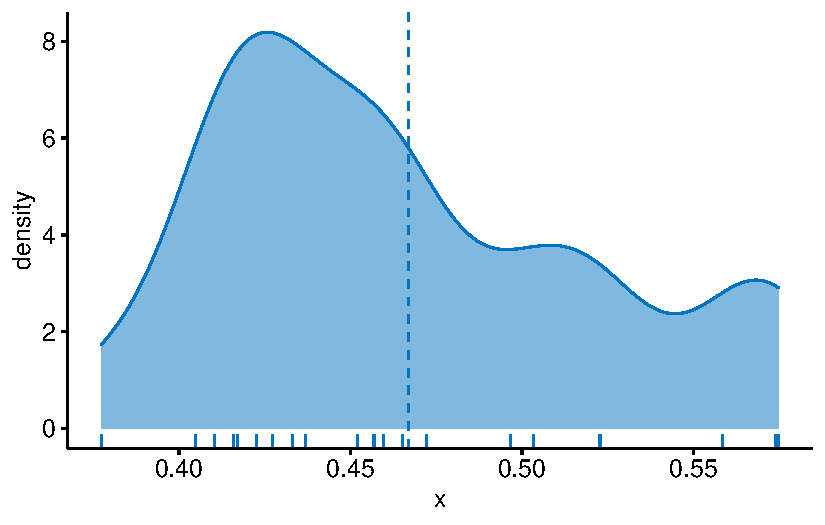
\includegraphics{Quarto_files/figure-pdf/unnamed-chunk-14-1.pdf}

}

\end{figure}

\begin{Shaded}
\begin{Highlighting}[]
\FunctionTok{library}\NormalTok{(forecast)}
\end{Highlighting}
\end{Shaded}

\begin{verbatim}
Warning: package 'forecast' was built under R version 4.1.3
\end{verbatim}

\begin{Shaded}
\begin{Highlighting}[]
\NormalTok{Tt }\OtherTok{\textless{}{-}} \FunctionTok{trendcycle}\NormalTok{(tdx.dcp)}
\NormalTok{St }\OtherTok{\textless{}{-}} \FunctionTok{seasonal}\NormalTok{(tdx.dcp)}
\NormalTok{Rt }\OtherTok{\textless{}{-}} \FunctionTok{remainder}\NormalTok{(tdx.dcp)}
\FunctionTok{plot}\NormalTok{(Tt)}
\end{Highlighting}
\end{Shaded}

\begin{figure}[H]

{\centering 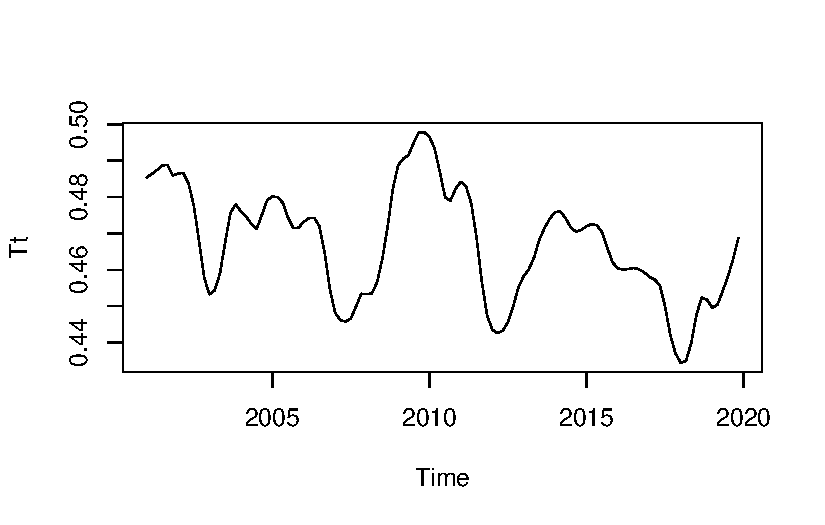
\includegraphics{Quarto_files/figure-pdf/unnamed-chunk-15-1.pdf}

}

\end{figure}

\begin{Shaded}
\begin{Highlighting}[]
\FunctionTok{plot}\NormalTok{(St)}
\end{Highlighting}
\end{Shaded}

\begin{figure}[H]

{\centering 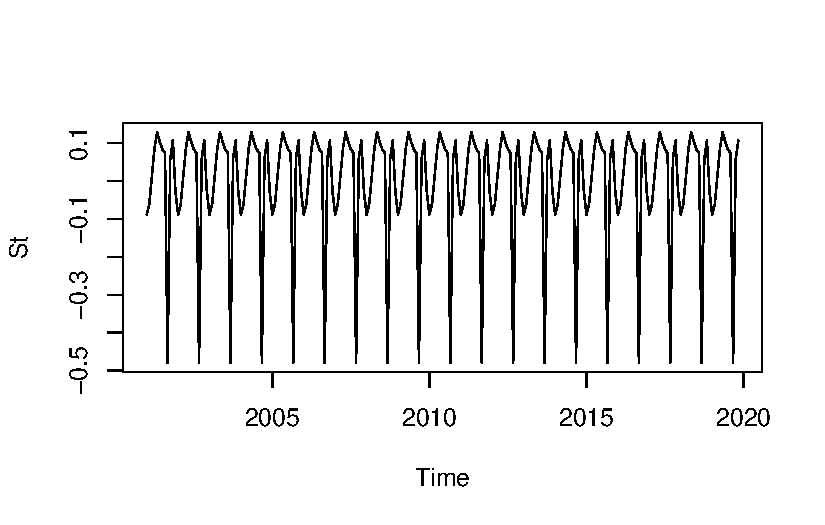
\includegraphics{Quarto_files/figure-pdf/unnamed-chunk-15-2.pdf}

}

\end{figure}

\begin{Shaded}
\begin{Highlighting}[]
\FunctionTok{plot}\NormalTok{(Rt)}
\end{Highlighting}
\end{Shaded}

\begin{figure}[H]

{\centering 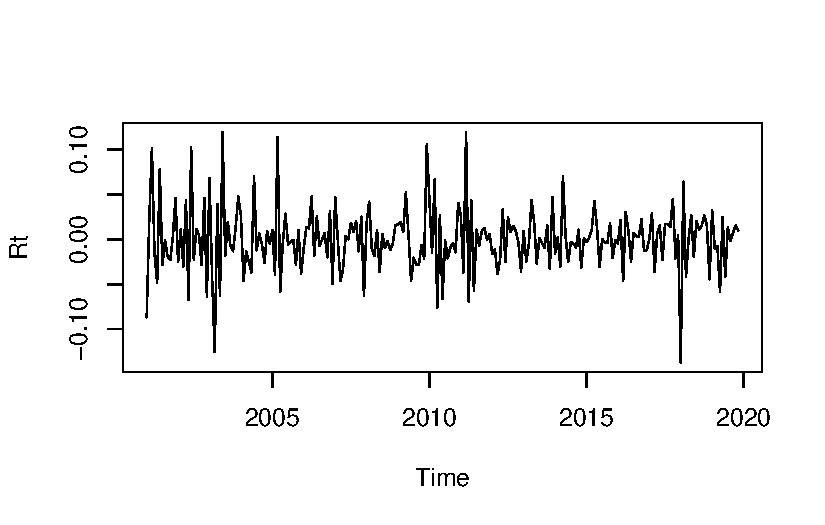
\includegraphics{Quarto_files/figure-pdf/unnamed-chunk-15-3.pdf}

}

\end{figure}

\hypertarget{section-1}{%
\section{}\label{section-1}}

When investigating a time series, one of the first things to check
before building an ARIMA model is to check that the series is
stationary. That is, it needs to be determined that the time series is
constant in mean and variance are constant and not dependent on time.

Here, we will look at a couple methods for checking stationarity. If the
time series is provided with seasonality, a trend, or a change point in
the mean or variance, then the influences need to be removed or
accounted for. Augmented Dickey--Fuller (ADF) t-statistic test to find
if the series has a unit root (a series with a trend line will have a
unit root and result in a large p-value).

\begin{Shaded}
\begin{Highlighting}[]
\FunctionTok{library}\NormalTok{(tseries)}
\FunctionTok{adf.test}\NormalTok{(Rt)}
\end{Highlighting}
\end{Shaded}

\begin{verbatim}

    Augmented Dickey-Fuller Test

data:  Rt
Dickey-Fuller = -8.639, Lag order = 6, p-value = 0.01
alternative hypothesis: stationary
\end{verbatim}

\begin{Shaded}
\begin{Highlighting}[]
\FunctionTok{adf.test}\NormalTok{(Tt)}
\end{Highlighting}
\end{Shaded}

\begin{verbatim}

    Augmented Dickey-Fuller Test

data:  Tt
Dickey-Fuller = -3.4545, Lag order = 6, p-value = 0.04798
alternative hypothesis: stationary
\end{verbatim}

\begin{Shaded}
\begin{Highlighting}[]
\FunctionTok{adf.test}\NormalTok{(tdx)}
\end{Highlighting}
\end{Shaded}

\begin{verbatim}

    Augmented Dickey-Fuller Test

data:  tdx
Dickey-Fuller = -8.2685, Lag order = 6, p-value = 0.01
alternative hypothesis: stationary
\end{verbatim}

\#Autocorrelation Function (ACF) Identify if correlation at different
time lags goes to 0

\begin{Shaded}
\begin{Highlighting}[]
\FunctionTok{plot.new}\NormalTok{()}
\FunctionTok{frame}\NormalTok{()}
\CommentTok{\# The Stationary Signal and ACF}
\FunctionTok{plot}\NormalTok{(Rt,}\AttributeTok{col=} \StringTok{"red"}\NormalTok{, }\AttributeTok{main =} \StringTok{"Stationary Signal"}\NormalTok{)}
\end{Highlighting}
\end{Shaded}

\begin{figure}[H]

{\centering 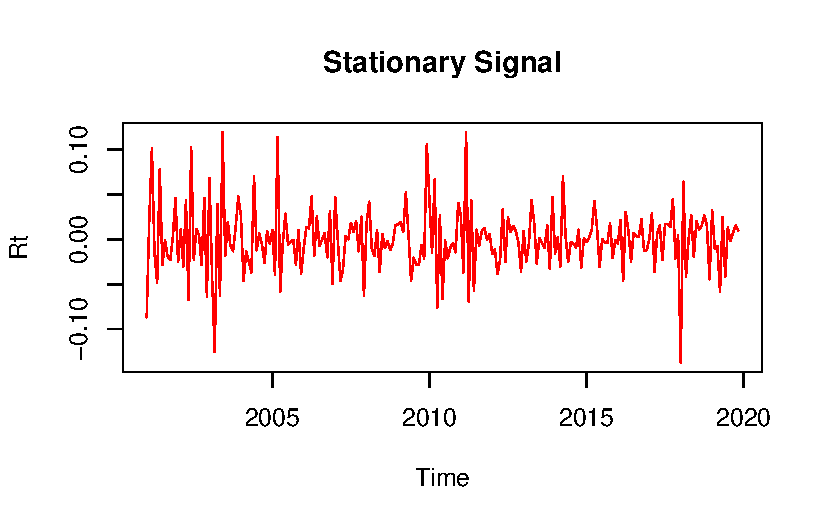
\includegraphics{Quarto_files/figure-pdf/unnamed-chunk-17-1.pdf}

}

\end{figure}

\begin{Shaded}
\begin{Highlighting}[]
\FunctionTok{acf}\NormalTok{(Rt, }\AttributeTok{lag.max =} \FunctionTok{length}\NormalTok{(Rt),}
    \AttributeTok{xlab =} \StringTok{"lag \#"}\NormalTok{, }\AttributeTok{ylab =} \StringTok{\textquotesingle{}ACF\textquotesingle{}}\NormalTok{, }\AttributeTok{main =} \StringTok{\textquotesingle{}\textquotesingle{}}\NormalTok{)}
\end{Highlighting}
\end{Shaded}

\begin{figure}[H]

{\centering 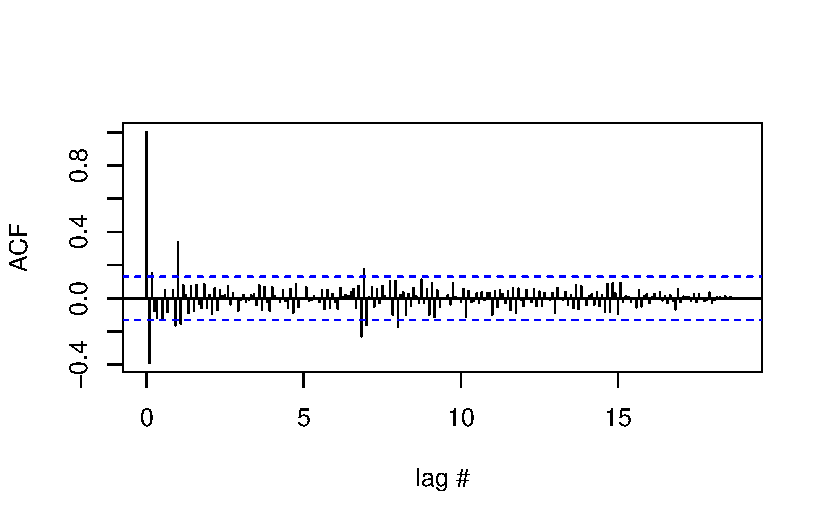
\includegraphics{Quarto_files/figure-pdf/unnamed-chunk-17-2.pdf}

}

\end{figure}

\begin{Shaded}
\begin{Highlighting}[]
\CommentTok{\#The Trend Signal anf ACF}

\FunctionTok{plot}\NormalTok{(Tt,}\AttributeTok{col=} \StringTok{"red"}\NormalTok{,}\AttributeTok{main =} \StringTok{"Trend Signal"}\NormalTok{)}
\end{Highlighting}
\end{Shaded}

\begin{figure}[H]

{\centering 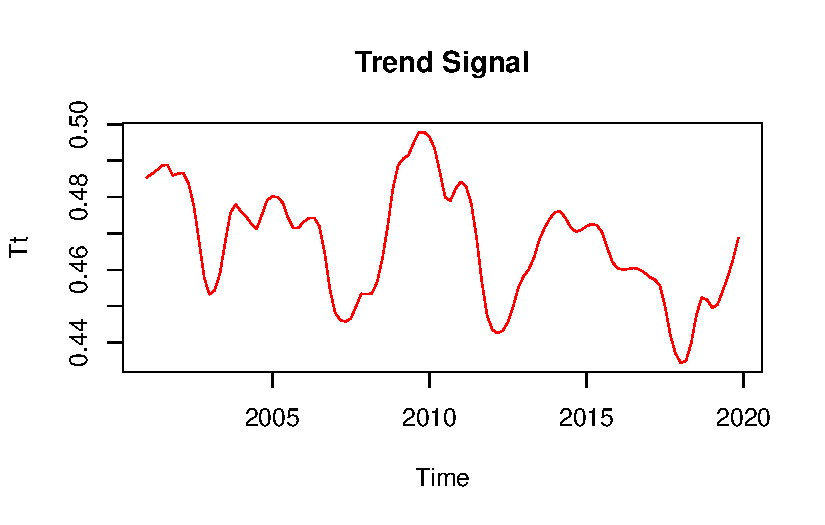
\includegraphics{Quarto_files/figure-pdf/unnamed-chunk-17-3.pdf}

}

\end{figure}

\begin{Shaded}
\begin{Highlighting}[]
\FunctionTok{acf}\NormalTok{(Tt, }\AttributeTok{lag.max =} \FunctionTok{length}\NormalTok{(Tt),}
    \AttributeTok{xlab =} \StringTok{"lag\#"}\NormalTok{, }\AttributeTok{ylab =} \StringTok{"ACF"}\NormalTok{, }\AttributeTok{main =} \StringTok{\textquotesingle{}\textquotesingle{}}\NormalTok{)}
\end{Highlighting}
\end{Shaded}

\begin{figure}[H]

{\centering 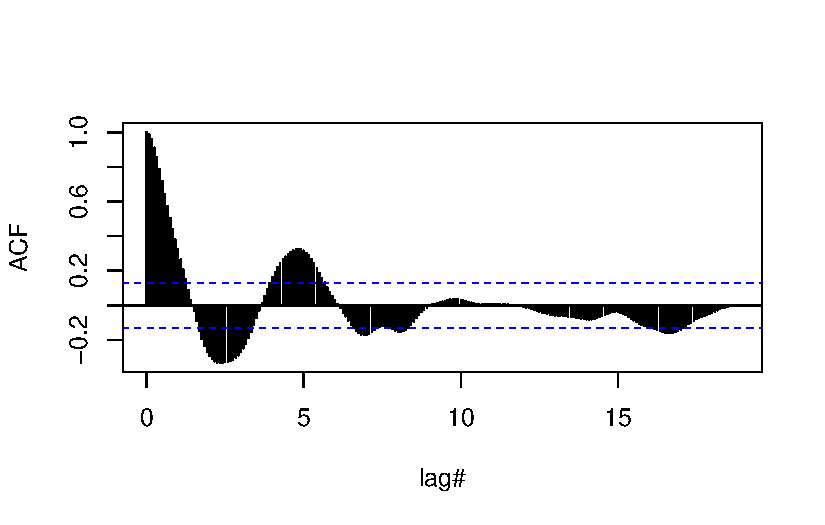
\includegraphics{Quarto_files/figure-pdf/unnamed-chunk-17-4.pdf}

}

\end{figure}

It is noteworthy that the stationary signal (top left) generates few
significant lags that are larger than the ACF's confidence interval
(blue dotted line, bottom left). In contrast, practically all delays in
the time series with a trend (top right) surpass the ACF's confidence
range (bottom right). Qualitatively, we can observe and infer from the
ACFs that the signal on the left is steady (due to the lags that die
out) whereas the signal on the right is not (since later lags exceed the
confidence interval).

\begin{Shaded}
\begin{Highlighting}[]
\NormalTok{tdx.ns }\OtherTok{\textless{}{-}} \FunctionTok{data.frame}\NormalTok{(}\AttributeTok{time =} \FunctionTok{c}\NormalTok{(}\DecValTok{1}\SpecialCharTok{:}\FunctionTok{length}\NormalTok{(tdx)), }\AttributeTok{trend =}\NormalTok{ tdx }\SpecialCharTok{{-}}\NormalTok{ tdx.dcp}\SpecialCharTok{$}\NormalTok{time.series[,}\DecValTok{1}\NormalTok{])}
\NormalTok{summary }\OtherTok{\textless{}{-}} \FunctionTok{summary}\NormalTok{(}\FunctionTok{lm}\NormalTok{(}\AttributeTok{formula =}\NormalTok{ trend }\SpecialCharTok{\textasciitilde{}}\NormalTok{ time, }\AttributeTok{data =}\NormalTok{ tdx.ns))}
\end{Highlighting}
\end{Shaded}

\begin{Shaded}
\begin{Highlighting}[]
\FunctionTok{plot}\NormalTok{(tdx.ns)}
\FunctionTok{abline}\NormalTok{(}\AttributeTok{a =}\NormalTok{ summary}\SpecialCharTok{$}\NormalTok{coefficients[}\DecValTok{1}\NormalTok{,}\DecValTok{1}\NormalTok{], }\AttributeTok{b =}\NormalTok{ summary}\SpecialCharTok{$}\NormalTok{coefficients[}\DecValTok{2}\NormalTok{,}\DecValTok{1}\NormalTok{], }\AttributeTok{col =} \StringTok{\textquotesingle{}blue\textquotesingle{}}\NormalTok{)}
\end{Highlighting}
\end{Shaded}

\begin{figure}[H]

{\centering 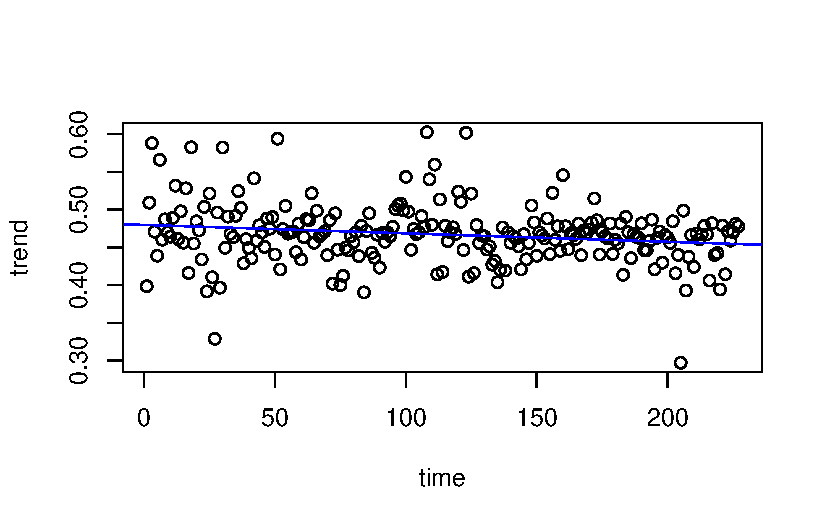
\includegraphics{Quarto_files/figure-pdf/unnamed-chunk-19-1.pdf}

}

\end{figure}

\begin{Shaded}
\begin{Highlighting}[]
\CommentTok{\# library(tidyverse)}
\CommentTok{\# devtools::install\_github("EvaMaeRey/ggxmean")}
\CommentTok{\# library(ggxmean)}
\CommentTok{\# }
\end{Highlighting}
\end{Shaded}

\begin{Shaded}
\begin{Highlighting}[]
\CommentTok{\# Count of na values to dataframe}
\CommentTok{\# Calculating Trend and Seasonal Strength}
\NormalTok{evi.trend}\SpecialCharTok{$}\NormalTok{NA\_Values[i] }\OtherTok{\textless{}{-}}\NormalTok{ na.cnt}
\NormalTok{evi.trend}\SpecialCharTok{$}\NormalTok{Trend[i] }\OtherTok{\textless{}{-}}\NormalTok{ summary}\SpecialCharTok{$}\NormalTok{coefficients[}\DecValTok{2}\NormalTok{,}\DecValTok{1}\NormalTok{]}
\NormalTok{evi.trend}\SpecialCharTok{$}\NormalTok{Trend\_Strength[i] }\OtherTok{\textless{}{-}} \FunctionTok{round}\NormalTok{(}\FunctionTok{max}\NormalTok{(}\DecValTok{0}\NormalTok{,}\DecValTok{1}\SpecialCharTok{{-}}\NormalTok{(}\FunctionTok{var}\NormalTok{(Rt)}\SpecialCharTok{/}\FunctionTok{var}\NormalTok{(Tt}\SpecialCharTok{+}\NormalTok{Rt))),}\DecValTok{1}\NormalTok{)}
\NormalTok{evi.trend}\SpecialCharTok{$}\NormalTok{Seasonal\_Strength[i] }\OtherTok{\textless{}{-}} \FunctionTok{round}\NormalTok{(}\FunctionTok{max}\NormalTok{(}\DecValTok{0}\NormalTok{,}\DecValTok{1}\SpecialCharTok{{-}}\NormalTok{(}\FunctionTok{var}\NormalTok{(Rt)}\SpecialCharTok{/}\FunctionTok{var}\NormalTok{(St}\SpecialCharTok{+}\NormalTok{Rt))),}\DecValTok{1}\NormalTok{)}
\NormalTok{evi.trend}\SpecialCharTok{$}\NormalTok{P\_value[i] }\OtherTok{\textless{}{-}}\NormalTok{ summary}\SpecialCharTok{$}\NormalTok{coefficients[}\DecValTok{2}\NormalTok{,}\DecValTok{4}\NormalTok{]}
\NormalTok{evi.trend}\SpecialCharTok{$}\NormalTok{R\_Squared[i] }\OtherTok{\textless{}{-}}\NormalTok{ summary}\SpecialCharTok{$}\NormalTok{r.squared}
\NormalTok{evi.trend}\SpecialCharTok{$}\NormalTok{Standard\_Error[i] }\OtherTok{\textless{}{-}}\NormalTok{ summary}\SpecialCharTok{$}\NormalTok{sigma}
\NormalTok{evi.trend[i,]}
\end{Highlighting}
\end{Shaded}

\begin{verbatim}
  hex_id na.cnt NA_Values       Trend     P_value  R_Squared Standard_Error
1     34      0       152 -0.00011184 0.005928196 0.03316554     0.03974499
  Trend_Strength Seasonal_Strength
1            0.2                 1
\end{verbatim}

\begin{Shaded}
\begin{Highlighting}[]
\FunctionTok{plot}\NormalTok{(evi.hw }\OtherTok{\textless{}{-}}\NormalTok{ forecast}\SpecialCharTok{::}\FunctionTok{hw}\NormalTok{(}\AttributeTok{y =}\NormalTok{ tdx, }\AttributeTok{h =} \DecValTok{12}\NormalTok{, }\AttributeTok{damped =}\NormalTok{ T))}
\end{Highlighting}
\end{Shaded}

\begin{figure}[H]

{\centering 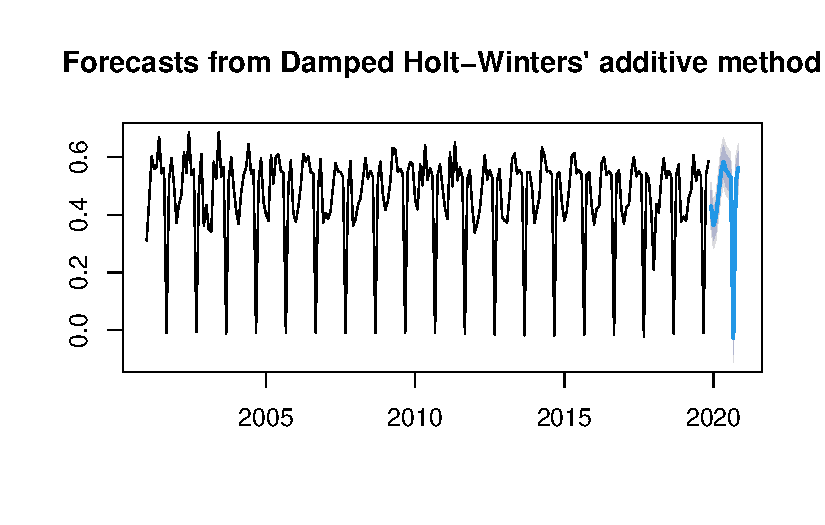
\includegraphics{Quarto_files/figure-pdf/unnamed-chunk-22-1.pdf}

}

\end{figure}

\begin{Shaded}
\begin{Highlighting}[]
\CommentTok{\#ggdensity(tdx, x = "tmie",y = "trend",fill = "\#0073C2FF",color ="\#0073C2FF",add = "mean",rug = TRUE)}
\end{Highlighting}
\end{Shaded}

\hypertarget{chapter-five}{%
\section{CHAPTER FIVE}\label{chapter-five}}

\hypertarget{conclusions-and-recommendations}{%
\subsection{CONCLUSIONS AND
RECOMMENDATIONS}\label{conclusions-and-recommendations}}

\hypertarget{summary}{%
\subsubsection{Summary}\label{summary}}

Broadly speaking, in this study we have presented a state-of-the-art of
the following popular time series forecasting models with their salient
features:

\begin{itemize}
\tightlist
\item
  The Box-Jenkins or ARIMA models for linear time series forecasting.
\item
  Some non-linear stochastic models, such as NMA, ARCH.
\item
  SVM based forecasting models; LS-SVM and DLS-SVM.
\end{itemize}

\hypertarget{conclusions}{%
\subsubsection{Conclusions}\label{conclusions}}

It has been seen that, the proper selection of the model orders (in case
of ARIMA), the number of input, hidden, output and the constant
hyper-parameters (in case of SVM) is extremely crucial for successful
forecasting. We have discussed the two important functions. AIC and BIC,
which are frequently used for ARIMA model selection.

We have considered a few important performance measures for evaluating
the accuracy of forecasting models. It has been understood that for
obtaining a reasonable knowledge about the overall forecasting error,
more than one measure should be used in practice. The last chapter
contains the forecasting results of our experiments, performed on six
real time series datasets. Our satisfactory understanding about the
considered forecasting models and their successful implementation can be
observed form the five performance measures and the forecast diagrams,
we obtained for each of the six datasets. However in some cases,
significant deviation can be seen among the original observations and
our forecast values. In such cases, we can suggest that a suitable data
preprocessing, other than those we have used in our work may improve the
forecast performances.

\hypertarget{recommendations}{%
\subsubsection{Recommendations}\label{recommendations}}

Time series forecasting is a fast growing area of research and as such
provides many scope for future works. One of them is the Combining
Approach, i.e.~to combine a number of different and dissimilar methods
to improve forecast accuracy. A lot of works have been done towards this
direction and various combining methods have been proposed in literature
{[}8, 14, 15, 16{]}. Together with other analysis in time series
forecasting, we have thought to find an efficient combining model, in
future if possible. With the aim of further studies in time series
modeling and forecasting

\hypertarget{references}{%
\subsection{References}\label{references}}


\printbibliography


\end{document}
